\documentclass[border=10pt]{standalone}
\usepackage[svgnames]{xcolor}
\usepackage{amsmath}
\usepackage{pgfplots}
\pgfplotsset{compat=newest}
\usepackage[sfdefault]{FiraSans}
\usepackage{FiraMono}
\renewcommand*\familydefault{\sfdefault}
\begin{document}
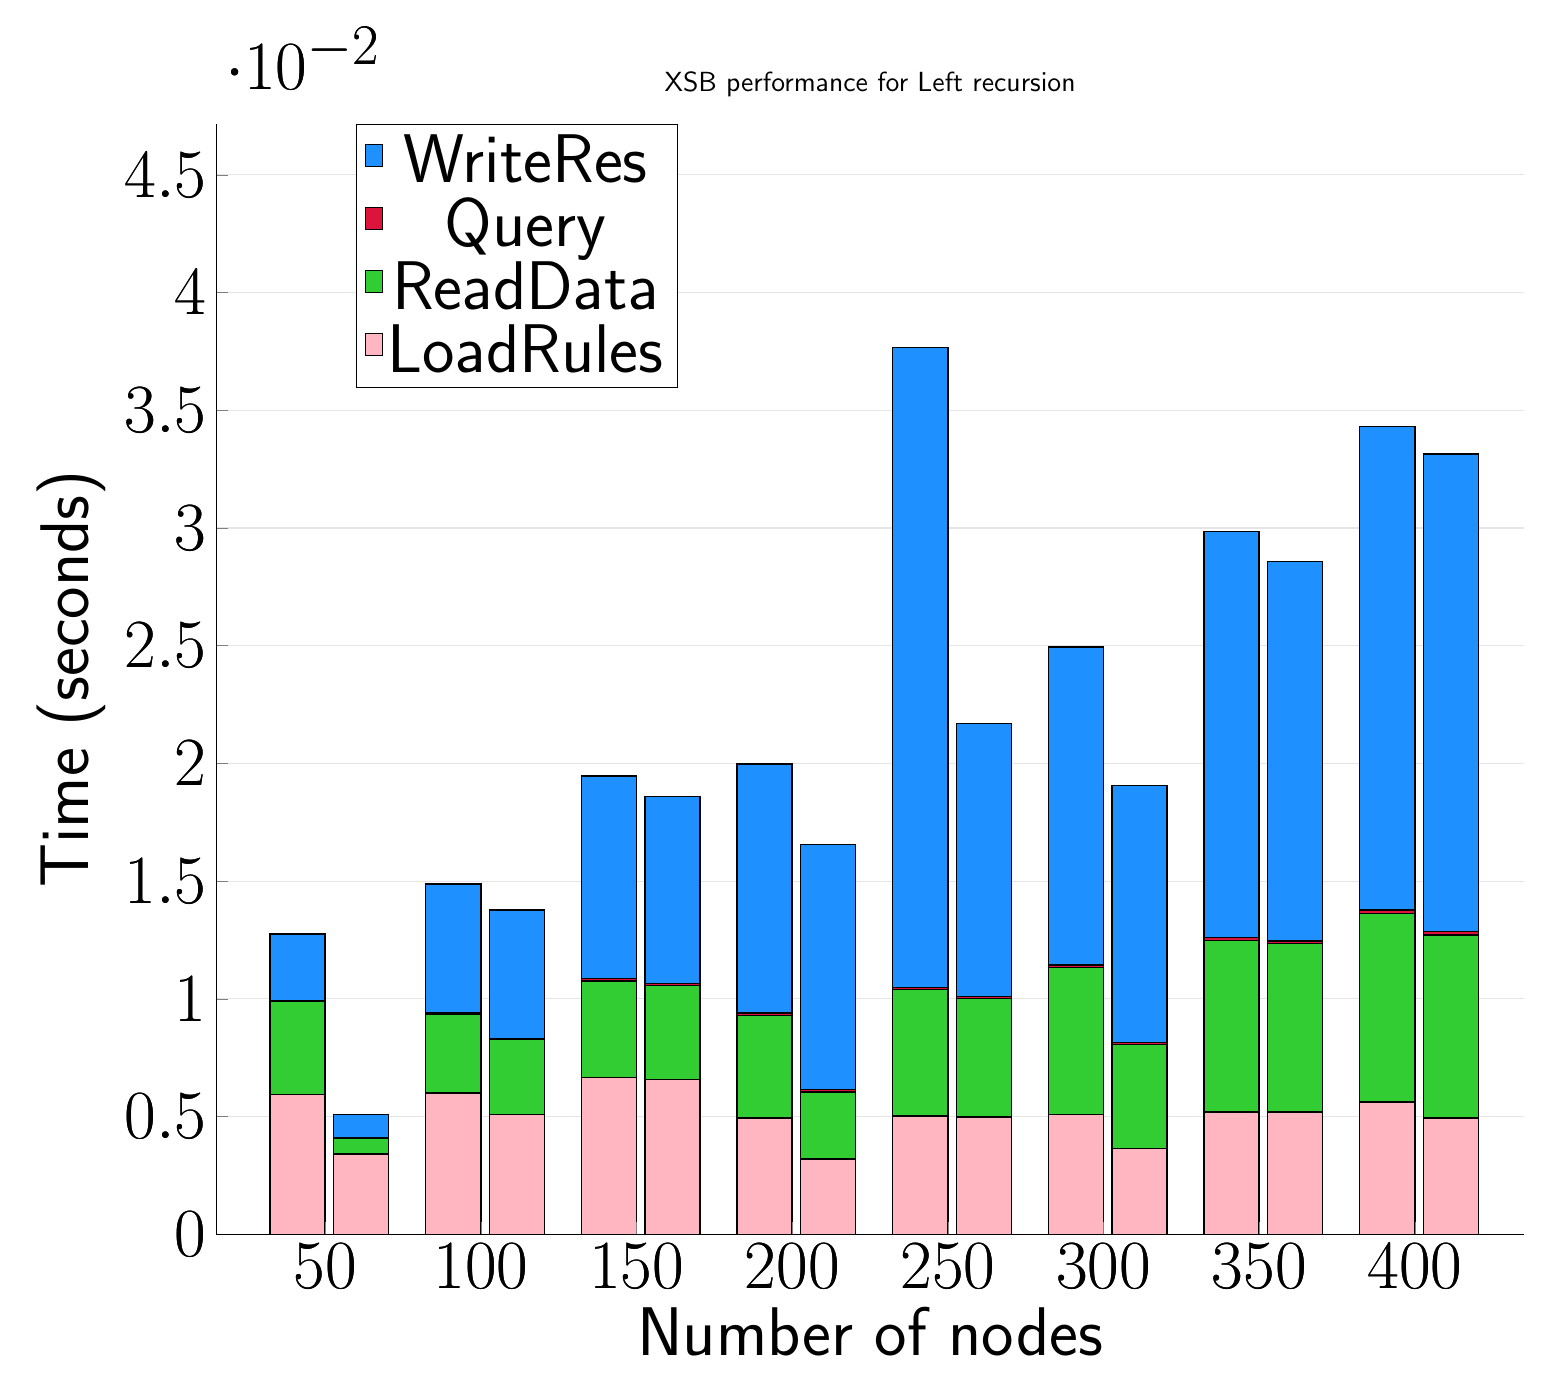
\begin{tikzpicture}
\begin{axis}[
   ybar stacked,
   title={XSB performance for Left recursion},
   bar shift=-10pt,
   width=1.5\textwidth,
   bar width=0.7cm,
   ymajorgrids, tick align=inside,
   major grid style={draw=gray!20},
   xtick=data,
   ymin=0, ymax=0.04718456586201984,
   axis x line*=bottom,
   axis y line*=left,
   enlarge x limits=0.1,
   legend style={
       at={(0.23, 1)},
       anchor=north,
       legend columns=1,
       font=\Huge,
   },
   ylabel={Time (seconds)},
   xlabel={Number of nodes},
   label style={font=\Huge},
   tick label style={font=\Huge},
]
\addlegendimage{fill=DodgerBlue, draw=black, line width=0.2pt}
\addlegendentry{WriteRes}
\addlegendimage{fill=Crimson, draw=black, line width=0.2pt}
\addlegendentry{Query}
\addlegendimage{fill=LimeGreen, draw=black, line width=0.2pt}
\addlegendentry{ReadData}
\addlegendimage{fill=LightPink, draw=black, line width=0.2pt}
\addlegendentry{LoadRules}
\addplot +[fill=LightPink, draw=black, line width=0.5pt] coordinates {
    (50, 0.00592652956644694)
    (100, 0.005994876225789387)
    (150, 0.006645441055297854)
    (200, 0.004929622014363603)
    (250, 0.005023956298828123)
    (300, 0.005090951919555667)
    (350, 0.0051879088083903)
    (400, 0.0056153933207194)
};
\addplot +[fill=LimeGreen, draw=black, line width=0.5pt] coordinates {
    (50, 0.0039474169413248736)
    (100, 0.0033613046010335297)
    (150, 0.0041162967681884766)
    (200, 0.004359324773152671)
    (250, 0.0053763389587402335)
    (300, 0.006229559580485026)
    (350, 0.007293065388997397)
    (400, 0.008020639419555662)
};
\addplot +[fill=Crimson, draw=black, line width=0.5pt] coordinates {
    (50, 4.569689432779946e-05)
    (100, 6.667772928873696e-05)
    (150, 9.393692016601577e-05)
    (200, 0.00010999043782552098)
    (250, 9.107589721679693e-05)
    (300, 0.000111738840738932)
    (350, 0.000125010808308919)
    (400, 0.0001393159230550133)
};
\addplot +[fill=DodgerBlue, draw=black, line width=0.5pt] coordinates {
    (50, 0.0028353532155354806)
    (100, 0.0054574012756347665)
    (150, 0.008611758550008139)
    (200, 0.010571956634521476)
    (250, 0.02718456586201984)
    (300, 0.013518015543619801)
    (350, 0.01724569002787275)
    (400, 0.020546436309814453)
};
\end{axis}
\begin{axis}[
   ybar stacked,
   bar shift=13pt,
   width=1.5\textwidth,
   bar width=0.7cm,
   ymajorgrids, tick align=inside,
   major grid style={draw=none},
   xtick=data,
   ymin=0, ymax=0.04718456586201984,
   axis x line*=none,
   axis y line*=none,
   enlarge x limits=0.1,
   label style={font=\Huge},
   tick label style={font=\Huge},
]
\addplot +[fill=LightPink, draw=black, line width=0.5pt] coordinates {
    (50, 0.0033996666666666667)
    (100, 0.005092666666666666)
    (150, 0.006569333333333333)
    (200, 0.0031886666666666665)
    (250, 0.004979666666666667)
    (300, 0.003637999999999999)
    (350, 0.005184999999999997)
    (400, 0.00493166666666667)
};
\addplot +[fill=LimeGreen, draw=black, line width=0.5pt] coordinates {
    (50, 0.0006920000000000042)
    (100, 0.0031666666666666666)
    (150, 0.004001666666666667)
    (200, 0.0028580000000000046)
    (250, 0.005025000000000007)
    (300, 0.004421999999999996)
    (350, 0.00715466666666667)
    (400, 0.007785333333333334)
};
\addplot +[fill=Crimson, draw=black, line width=0.5pt] coordinates {
    (50, 1.59999999999975e-05)
    (100, 6.533333333333159e-05)
    (150, 9.233333333333317e-05)
    (200, 9.733333333332904e-05)
    (250, 8.299999999999513e-05)
    (300, 8.866666666666744e-05)
    (350, 0.00012399999999999667)
    (400, 0.00013799999999999902)
};
\addplot +[fill=DodgerBlue, draw=black, line width=0.5pt] coordinates {
    (50, 0.0009703333333333357)
    (100, 0.005445666666666668)
    (150, 0.007921333333333338)
    (200, 0.010418666666666672)
    (250, 0.011607000000000004)
    (300, 0.010902666666666666)
    (350, 0.016127000000000002)
    (400, 0.020295333333333332)
};
\end{axis}
\end{tikzpicture}

\end{document}
